% !TEX root = ../thesis.tex

\chapter{Identifying Repeated Eigendirections in Manifold Learning \label{ch:harmonics}}

\graphicspath{{ch-harmonics/figures/}}

{\em This work is currently being prepared for publication.}


\section{Introduction}

As discussed in previous chapters, in recent years, manifold learning algorithms have proven useful for many disciplines and applications \cite{gepshtein2013image, fernandez2014diffusion, singer2011viewing, yuan2014automated, zhao2003face, trapnell2014dynamics, kemelmacher2011exploring, sifre2013rotation}, especially when no simple analytical model exists to describe the underlying dynamics.
%
%In particular, for dynamical systems, data-driven methodologies are essential when a simple macroscopic model cannot be written analytically due to the complexity of the system \cite{talmon2014intrinsic,berry2013time,singer2009detecting,ferguson2010systematic}.
%%
%For simulations, the governing model is often very high-dimensional and the macroscale dynamics are not obvious; for experimental systems, an explicit model is often unknown.
%%
%For such cases, data obtained from observations and/or simulations of the dynamical system combined with such methodologies gives rise to a low-dimensional description which can not only provide insight into the underlying dynamics, but also serve as a first step in constructing macroscale models which are consistent with the observed microscale behavior.
%
%Due to the complexity and range of microscale behaviors possible in dynamical systems, we use manifold learning, a class of nonlinear data-driven techniques, to analyze data.
%%
%Most manifold learning algorithms construct parametrizations of the data through the spectral analysis of a Laplace operator \cite{Belkin2003,coifman2005geometric,coifman2006geometric,singer2008non}.
%%
%The data is then embedded in a new, low-dimensional coordinate system given by the eigenvectors of this operator.
%%
%Our hope is that these coordinates, obtained in a data-driven manner, will describe the variables which govern the macroscale dynamical behavior of the system and enable us to introduce a reduced macroscale {\em ab initio} model.
%
These manifold learning algorithms were first applied to synthetic data sets to illustrate their geometric properties and flexibility \cite{coifman2005geometric, nadler2006diffusion}.
%
Only recently have they been applied to experimental and simulation data, which was possible due to advances in data representation (observers) and metrics \cite{rubner2000earth,mallat2012group,talmon2013empirical,zhao2014rotationally, rohrdanz2011determination}.
%
A critical shortcoming of these methods is that from a geometric perspective, not all eigenvectors are guaranteed to parametrize unique directions within the data; some eigenvectors are ``repeated eigendirections'' which describe the same mode.
%
Identifying those eigenvectors is critical for obtaining a parametrization of the system which captures the true dimensionality of the macroscale dynamics.
%
This is a challenging task which is often done manually, and few methods have been proposed to automate the identification of the unique eigendirections \cite{gerber2007robust}.

In this paper, we propose an algorithm to automatically identify the unique eigendirections using local linear regression \cite{wasserman2006all}.
%
We first demonstrate our algorithm on synthetic examples where a closed-form solution for the eigenvectors and eigenvalues of the Laplace operator is known, which will allow us to validate our proposed approach.
%
We then consider a complex data set from a stochastic dynamical system simulation which models cellular chemotaxis \cite{othmer1988models}.
%
The recent advances in observers and metrics, coupled with the proposed approach for identifying the unique eigendirections, provide a data analysis pipeline which successfully analyzes data from this simulation in a purely data-driven manner.
%
We will show that this pipeline allows us to detect changes in the regime/mode of the system, as well as changes in the underlying dimensionality of the macroscale dynamics.


\section{Manifold Learning Based on Laplace Operators}
%Although data from dynamical systems is often high-dimensional, since it is collected at the microscale, the macroscale dynamics often evolve to a low-dimensional description.
%
%In such cases, the high-dimensional microscale data is restricted to a low-dimensional manifold embedded in the high-dimensional space, and extracting a parametrization of this manifold corresponds to parametrizing the low-dimensional, macroscale dynamics.
%

Let $\data(1), \dots, \data(m) \in \mathbb{R}^\highdim$ denote $\ndata$ observations sampled from the dynamical system.
%
We assume the $\highdim$-dimensional observations $\data(i)$ lie on a $\lowdim$-dimensional manifold $\manifold$, where $\lowdim < \highdim$.
%
We therefore consider the problem of parametrizing the continuous $d$-dimensional manifold $\manifold$ embedded in $\mathbb{R}^\highdim$ from data.
%
For linear hyperplanes, the principal axes parametrize the manifold.
%
However, in the case when the manifold is nonlinear, the set of coordinates is not readily apparent.
%
By using a particular manifold learning technique based on the construction of a Laplace operator, namely, diffusion maps, we will show how to extract a $\lowdim$-dimensional parametrization of the observations which is consistent with the geometry of the manifold \cite{Belkin2003, coifman2005geometric, singer2008non}.

\subsection{Eigenfunctions of the Laplace-Beltrami operator}

\begin{figure}[t]
\centering
\begin{subfigure}{0.3\textwidth}
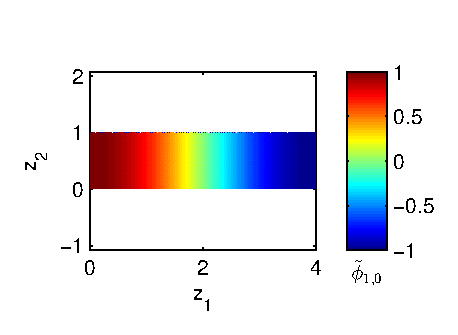
\includegraphics[width=\textwidth]{strip_cnts1}
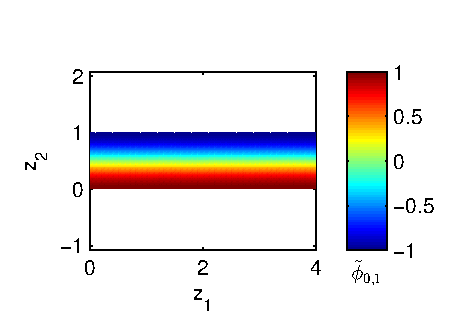
\includegraphics[width=\textwidth]{strip_cnts2}
\caption{}
\label{subfig:strip_efuncs}
\end{subfigure}
%
\begin{subfigure}{0.3\textwidth}
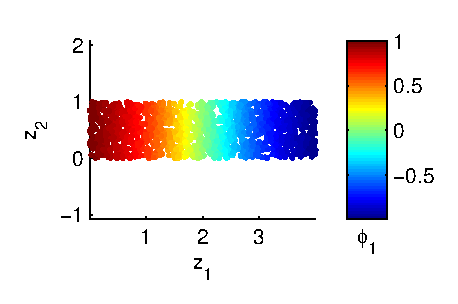
\includegraphics[width=\textwidth]{strip_discrete1}
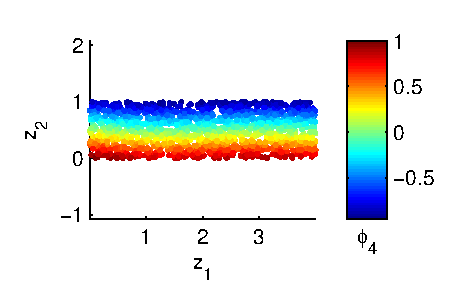
\includegraphics[width=\textwidth]{strip_discrete4}
\caption{}
\label{subfig:strip_evecs_uniform}
\end{subfigure}
%
\begin{subfigure}{0.3\textwidth}
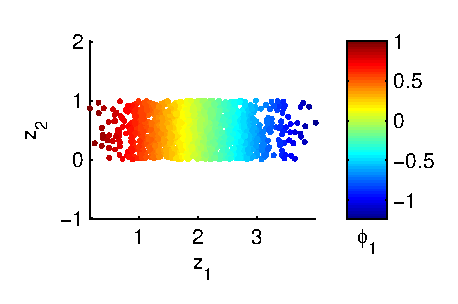
\includegraphics[width=\textwidth]{strip_nonuniform1}
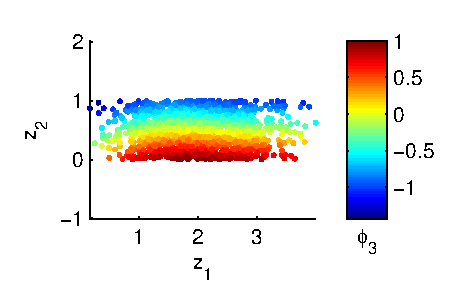
\includegraphics[width=\textwidth]{strip_nonuniform2}
\caption{}
\label{subfig:strip_evecs_nonuniform}
\end{subfigure}
%
\caption[Eigenfunctions of the Laplace-Beltrami operator on a two-dimensional strip]{(a) Two-dimensional continuous strip colored by the eigenfunctions $\tilde{\phi}_{1, 0} = \cos \left( {\pi z_1}/{L_1} \right)$, and $\tilde{\phi}_{0, 1} = \cos \left( {\pi z_2}/{L_2} \right)$. (b) Two-dimensional strip with uniform sampling colored by the first and fourth (non-trivial) eigenvectors of the discrete Laplacian. (c) Two-dimensional strip with data sampled from a Gaussian distribution in $z_1$ and sampled uniformly in $z_2$, colored by the first and third (non-trivial) eigenvectors of the discrete Laplacian. Note that in all cases we uncover parametrizations which are one-to-one with $z_1$ and $z_2$.}
\end{figure}

In recent years, it has been noted that the eigenfunctions of the \emph{continuous} Laplace-Beltrami operator provide ``good" coordinates for the manifold \cite{jones2008}.
%
Thus, we start by considering a continuous setting where rigorous analysis is available for specific examples.
%
Using such an example, we will show that the existence of repeated eigendirections is inherent to the manifold learning setup based on Laplace operators, and that the identification of the unique eigendirections is nontrivial.
%
The existence of these challenges in the continuous setting implies that, even in the limit of infinite data, such repeated eigendirections still pose a problem for analysis.

To illustrate why these eigenfunctions provide appropriate coordinates, consider a two-dimensional strip with edge lengths $L_1$ and $L_2$.
%
The eigenvalues of the Laplace-Beltrami operator with Neumann boundary conditions are given by
\begin{equation} \label{eq:evals}
\tilde{\lambda}_{k_1, k_2} = \left( \frac{k_1 \pi}{L_1} \right)^2 + \left( \frac{k_2 \pi}{L_2} \right)^2
\end{equation}
for $k_1, k_2 = 0, 1, 2, \dots$,
and the corresponding eigenfunctions are
\begin{equation} \label{eq:efuncs}
\tilde{\phi}_{k_1, k_2} = \cos \left( \frac{k_1 \pi z_1}{L_1} \right) \cos \left( \frac{k_2 \pi z_2}{L_2} \right)
\end{equation}
where $z_1$ and $z_2$ denote the two coordinates of the strip \cite{singer2008non}.
%
We note that the eigenfunctions $\tilde{\phi}_{1, 0} = \cos \left( {\pi z_1}/{L_1} \right)$ and $\tilde{\phi}_{0, 1} = \cos \left( {\pi z_2}/{L_2} \right)$ are one-to-one with the $z_1$ and $z_2$ coordinates, respectively, and therefore yield a parametrization of the underlying manifold (see Figure~\ref{subfig:strip_efuncs}).
%
Furthermore, the corresponding eigenvalues $\tilde{\lambda}_{1,0}$ and $\tilde{\lambda}_{0,1}$ provide a measure of $L_1$ versus $L_2$: as the ratio between $L_1$ and $L_2$ increases, the gap between $\tilde{\lambda}_{1,0}$ and $\tilde{\lambda}_{0,1}$ also increases (this will be discussed further in Section~\ref{sec:relative_lengths}).
%
The analytic form of the eigenfunctions in \eqref{eq:efuncs} illustrates the two issues we address in this paper.
%
First, $z_1$ and $z_2$ are not necessarily decoupled in subsequent eigenfunctions, and a proper parameterization of the manifold is not necessarily given by the $d$ eigenfunctions associated with the smallest $d$ eigenvalues.
% TODO: address this in later section
%
Second, eigenfunctions with $k_1+k_2 \ge 2$ do not describe any additional directions along the strip; we will refer to these as ``repeated eigendirections,'' and we will refer to the eigenfunctions with $k_1+k_2 =1$ as ``unique eigendirections.'' 
%
We note that, although the eigenfunctions can only be written analytically for very special cases, it has been observed empirically that the eigenfunctions often provide appropriate coordinates to parametrize more complex, nonlinear manifolds.
%
In addition, this problem of repeated eigendirections arises for more complex manifolds with more than two variables.


\subsection{Discrete approximation of the Laplace-Beltrami operator: diffusion maps}

In most applications, we are not given a description of the continuous manifold.
%
Instead, we are given data {\em sampled} from the underlying manifold, and the parameterization of the manifold needs to be uncovered from the data.
%
As discussed in \chap~\ref{ch:math}, diffusion maps constructs a matrix which, in the limit of infinite data, approximates the Laplace-Beltrami or Fokker-Planck operator on the manifold.
%
%It was shown in \cite{coifman2006geometric} that, in the limit of infinite data, this discrete Laplacian matrix constructed from data converges pointwise to the continuous Laplace-Beltrami operator on the manifold.
%%
%As a result, the eigenvectors of the discrete Laplacian approximate the eigenfunctions of this continuous operator.
%
%Given observations $z(1), \dots, z(m) \in \mathcal{M}_d$, we first construct the weight matrix $\mathbf{W} \in \mathbb{R}^{m \times m}$, with
%\begin{equation} \label{eq:W}
%\mathbf{W}_{ij} = \exp \left( -\frac{\|z(i) - z(j) \|^2}{\epsilon^2} \right), \ i,j=1,\ldots,m,
%\end{equation}
%where $\| \cdot \|$ denotes the appropriate norm for the observations, and $\epsilon$ is a characteristic distance between the observations.
%%
%The kernel's scale $\epsilon$ can be chosen using several heuristics \cite{rohrdanz2011determination, coifman2008graph}; we often take $\epsilon$ to be the median of the pairwise distances between the data points.
%%
%We then construct the diagonal matrix $\mathbf{D} \in \mathbb{R}^{m \times m}$, with $\mathbf{D}_{ii} = \sum_j \mathbf{W}_{ij}$, and form the matrix $\widetilde{\mathbf{W}} = \mathbf{D}^{-\alpha} \mathbf{W} \mathbf{D}^{-\alpha}$, where $0 < \alpha < 1$. 
%%
%Next, we construct the diagonal matrix $\widetilde{\mathbf{D}} \in \mathbb{R}^{m \times m}$, with $\widetilde{\mathbf{D}}_{ii} = \sum_j \widetilde{\mathbf{W}}_{ij}$, and the matrix $\mathbf{A}  = \widetilde{\mathbf{D}}^{-1} \widetilde{\mathbf{W}}.$
%
%If the data $z(1), \dots, z(m)$ are sampled from $\mathcal{M}_d$ with some density $q$, then, for $\epsilon \rightarrow 0, m \rightarrow \infty$, the discrete matrix convergences to the following continuous limit operators with Neumann boundary conditions (as discussed in the previous section) \cite{coifman2006geometric}
%\begin{align}
%\frac{1}{\epsilon^2}(\mathbf{I}-\mathbf{A}) \phi &\rightarrow \nabla^2 \phi - 2\nabla U \cdot \nabla \phi, &&\alpha = 0 \\
%\frac{1}{\epsilon^2}(\mathbf{I}-\mathbf{A}) \phi &\rightarrow \nabla^2 \phi - \nabla U \cdot \nabla \phi, &&\alpha = 1/2 \\
%\frac{1}{\epsilon^2}(\mathbf{I}-\mathbf{A}) \phi &\rightarrow \nabla^2 \phi, &&\alpha = 1
%\end{align}
%where $U = - \log q$.
%%
%The different limit operators, depending on the choice of $\alpha$, imply that nonuniform sampling on the manifold may have different effects. 
%%
%In particular, by setting $\alpha=1$, one can factor out the density effects in the weight matrix, and the discrete Laplacian matrix approaches the Laplace-Beltrami operator on the manifold $\mathcal{M}_d$.
%%
The eigenvectors $\phi_0, \phi_1, \dots, \phi_{\ndata-1}$ of $\mathbf{A}$ approximate the eigenfunctions of the Laplace-Beltrami operator on $\manifold$,
and the eigenvalues $\lambda_0, \lambda_1, \dots, \lambda_{\ndata-1}$ of $\mathbf{A}$ are related to the eigenvalues of the continuous operator by
\begin{equation} \label{eq:evals_relationship}
\lambda_k = \exp \left( -\frac{\epsilon^2}{4} \tilde{\lambda}_{k_1, k_2}  \right).
\end{equation}
%
%As discussed previously, the eigenfunctions provide a parametrization of the manifold, such that $\lambda_j^\tau \phi_{j}(i)$ yields the $j^{th}$ embedding coordinate for $z(i)$, where $\tau \ge 0$ is a parameter (in our examples, we will take $\tau=0$).
%%
%This is the standard diffusion maps embedding \cite{coifman2005geometric, coifman2006geometric}, where we order the eigenvectors such that $|\lambda_0| \ge |\lambda_1| \ge \dots \ge |\lambda_{m-1}|$.
%%
%Because the matrix $\mathbf{A}$ is row-stochastic ($\sum_j \mathbf{A}_{ij} = 1$),  $\lambda_0 = 1$ and $\phi_0$ is a trivial constant vector.
%%
%The distance induced by this mapping is called the standard diffusion distance,
%%
%\begin{equation}
%D^2_\tau(z(i), z(j)) = \sum_{k=1}^{m-1} \lambda_k^{2 \tau} \left( \phi_k(i) - \phi_k(j)  \right)^2.
%\end{equation}
%%
Figures~\ref{subfig:strip_evecs_uniform}--\ref{subfig:strip_evecs_nonuniform} shows data sampled from a strip, colored by eigenvectors of $\mathbf{A}$.
%
In cases of both uniform and nonuniform sampling, the selected eigenvectors are one-to-one with $z_1$ and $z_2$, and thus parametrize the manifold.
%
TODO: maybe we can put here the new figures for the different values of $\alpha$ instead of these figures.
%
Although we have considered a very simple example for illustrative purposes, common practice is to use these tools for high-dimensional, nonlinear data sets.

From the previous section, we know that the eigenfunctions with $(k_1, k_2) =(1, 0)$ and $(k_1, k_2) =(0, 1)$ provide embedding coordinates for the manifold; these two eigenfunctions are both uncoupled and not repeated.
%
From \eqref{eq:evals}, we see that sorting the eigenvectors by the magnitude of the corresponding eigenvalues implies that these two eigenvectors are guaranteed to appear before any coupled or repeated eigendirections.
%
However, these eigenvectors are {\em not} guaranteed to appear as the first two (non-trivial) eigenvectors, as harmonics of the first eigendirection (i.e., $\cos \left( n \pi z_1 / L_1 \right)$ with $n > 1$) could appear before the second.
%
We note that, in contrast to our simple illustrative example, for most data sets of interest, the coordinates for the underlying manifold are unknown and cannot easily be obtained from the coordinates of the original data, and identifying which eigenvectors correspond to unique eigendirections is nontrivial.

\section{Identifying the Informative Eigenvectors }

Common practice is to order the eigenvectors by the magnitude of the corresponding eigenvalues, assuming that the leading eigenvectors provide a parametrization of the underlying manifold.
%
However, as discussed in the previous section, some eigenvectors are higher harmonics of previous eigenvectors and do not describe new directions in the data set \cite{gerber2007robust}.
%
For the case where $\manifold$ is a $2$-dimensional strip with edge lengths $L_1  > L_2$, recall that the eigenfunctions $\tilde{\phi}_{1,0} = \cos \left(  {\pi z_1}/{L_1} \right)$ and  $\tilde{\phi}_{0,1} = \cos \left(  {\pi z_2}/{L_2} \right)$ provide embedding coordinates for the manifold $\mathcal{M}_d$.
%
However, these two eigenvectors $\tilde{\phi}_{1, 0}$ and $\tilde{\phi}_{0, 1}$ are not guaranteed to correspond to the two smallest (non-trivial) eigenvalues (the smallest eigenvalue will always be $\tilde{\lambda}_{0,0} = 0$ and correspond to a constant eigenfunction; these eigenvalues are related to the eigenvalues $\lambda_k$ of the discrete operator via \eqref{eq:evals_relationship}).
%
In fact, if $L_1 > 2 L_2$, then $\tilde{\lambda}_{2, 0} < \tilde{\lambda}_{0, 1}$, and so the second (non-trivial) eigenvector (when the eigenvectors are ordered by their corresponding eigenvalues) will be a repeated eigendirection of the first and still parametrize $z_1$ (see Figure~\ref{fig:strip_harmonics}).
%
We therefore require a methodology to automatically detect which eigenvectors are harmonics of each other.
%
Utilizing only the eigenvectors $\phi_i$ which correspond to unique eigendirections yields the most parsimonious representation of the data.
%
We will show how we can automatically detect these eigenvectors to obtain a meaningful representation of the data, and using only these eigenvectors yields a reduced embedding which is equivalent to the standard diffusion maps embedding.
%
Furthermore, the corresponding eigenvalues provide us with a measure of the relative lengths of the data set along these unique eigendirections.


\subsection{Algorithm: local linear regression}

\begin{figure}[t]
\centering
\begin{subfigure}{0.24\textwidth}
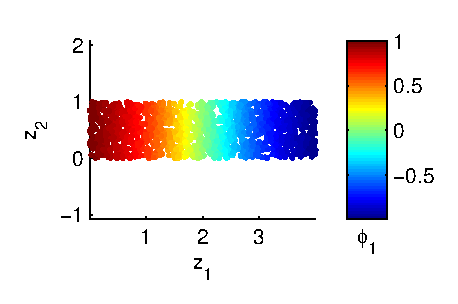
\includegraphics[width=\textwidth]{strip_discrete1}
\end{subfigure}
%
\begin{subfigure}{0.24\textwidth}
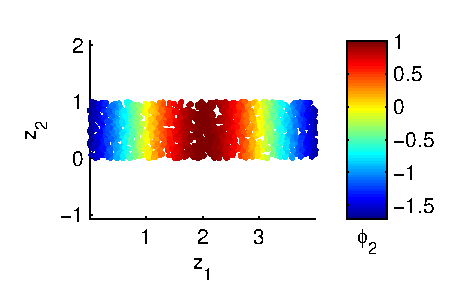
\includegraphics[width=\textwidth]{strip_discrete2}
\end{subfigure}
%
\begin{subfigure}{0.24\textwidth}
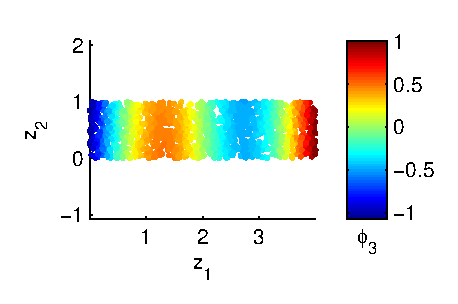
\includegraphics[width=\textwidth]{strip_discrete3}
\end{subfigure}
%
\begin{subfigure}{0.24\textwidth}
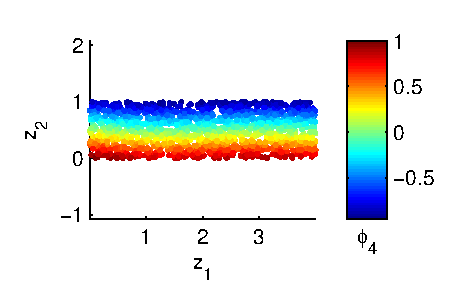
\includegraphics[width=\textwidth]{strip_discrete4}
\end{subfigure}
\caption[Eigenvectors of the discrete Laplacian on a two-dimensional strip]{Two-dimensional strip with uniform sampling colored by the first four (non-trivial) eigenvectors from diffusion maps. Note that the first and fourth eigenvectors are one-to-one with $z_1$ and $z_2$, respectively. However, the second and third eigenvectors are higher harmonics of the first eigenvector and do not capture any additional structure within the data set. }
\label{fig:strip_harmonics}
\end{figure}


Given the eigenvectors $\phi_1, \phi_2, \dots, \phi_{\ndata-1} \in \mathbb{R}^\ndata$, we would like to automatically deduce which ones capture new directions in the data, and which ones are merely repeated eigendirections.
%
This problem was addressed previously in \cite{gerber2007robust} by performing successive iterations of diffusion maps, interspersed with advection along the first eigendirection at each iteration.
%
However, this algorithm is somewhat {\em ad hoc}, and both the advection procedure and the successive eigendecompositions are very expensive and intractable for larger data set.
%TODO: elaborate on their method and find other advantages of our proposed method (for example, theirs is ad hoc).
%
Here, we propose an alternative approach to address the problem of repeated eigendirections.
%
Our approach is motivated by simple trigonometric arguments, such as the fact that $\cos2x$ (a repeated eigendirection) can be written as a function of $\cos x$ (a unique eigendirection).
%
We therefore attempt to fit a function $f(\phi_1, \dots, \phi_{k-1})$ to $\phi_{k}$; if the resulting fit is accurate, we assume $\phi_{k}$ is a repeated eigendirection of $\phi_1, \dots, \phi_{k-1}$.
%
We use a local linear function
\begin{equation}
\phi_k \approx \alpha + \beta^T \Phi_{k-1}
\end{equation}
%
as our functional approximation, where
%
$\Phi_{k-1} = \begin{bmatrix} \phi_1 & \dots & \phi_{k-1} \end{bmatrix}^T$,
$\alpha \in \mathbb{R}$, and $\beta \in \mathbb{R}^{k-1}$.
%
The coefficients $\alpha$ and $\beta$ are functions of $\Phi_{k-1}$ because we use a {\em local} linear fit in the $k-1$-dimensional $\Phi_{k-1}$ space, and so the coefficients change as a function of the domain.

At each point $\Phi_{k-1}(i)$, we approximate $\phi_k(i)$ by fitting a local linear function using the remaining $m-1$ data points.
%
We solve the following optimization problem
\begin{equation} \label{eq:opt_problem}
\hat{\alpha}_k (i) , \hat{\beta}_k(i)  = \argmin_{\alpha, \beta} \sum_{j \ne i} K(\Phi_{k-1}(i), \Phi_{k-1}(j)) \left( \phi_{k}(j) - (\alpha + \beta^T \Phi_{k-1}(j)) \right)^2.
\end{equation}
%
where $K$ is a kernel weighting function.
%
We use a Gaussian kernel,
%
\begin{equation}
K(\Phi_{k-1}(i), \Phi_{k-1}(j))  = \exp \left( - \frac{\|\Phi_{k-1}(i) - \Phi_{k-1} (j) \|^2}{\epsilon_{reg}^2} \right),
\end{equation}
%
where $\epsilon_{reg}$ is the kernel scale.
%
We typically take $\epsilon_{reg} = M / 3$, where $M$ is the median of the pairwise distances between $\Phi_{k-1}(i)$, as we empirically found this choice to yield good results.
%
We then define the normalized leave-one-out cross-validation error for this local linear fit as
\begin{equation} \label{eq:cv_error}
r_{k} = \sqrt{ \frac{\sum_{i=1}^n \left( \phi_{k} (i) - (\hat{\alpha}_k(i) + \hat{\beta}_k(i)^T \Phi_{k-1}(i))  \right)^2} {\sum_{i=1}^n  \left( \phi_{k} (i) \right)^2 }}.
\end{equation}
%
Note that a small value of $r_k$ implies that $\phi_{k}$ can be accurately approximated from $\phi_1, \dots, \phi_{k-1}$.
%
We assume small value of $r_k$ implies that $\phi_k$ is a harmonic of previous modes, i.e., a repeated eigendirection, and conversely, a large value of $r_{k}$ indicates that $\phi_{k}$ parametrizes a unique eigendirection in the data.
%
We choose to set $r_1 = 1$.
%
The error in \eqref{eq:cv_error} can easily be computed (see Section~5.4 of \cite{wasserman2006all}; code is also available at ...).

%The error in \eqref{eq:cv_error} can easily be computed \cite{wasserman2006all}.
%%
%We begin by constructing the matrix
%\begin{equation}
%X_{k-1}(i) = \begin{bmatrix}
%1 & \phi_1(1) - \phi_1(i) & \dots & \phi_{k-1}(1)- \phi_{k-1}(i) \\
%1 & \phi_1(2) - \phi_1(i) & \dots & \phi_{k-1}(2)- \phi_{k-1}(i) \\
%\vdots & \vdots & \ddots & \vdots \\
%1 & \phi_1(m) - \phi_1(i) & \dots & \phi_{k-1}(m)- \phi_{k-1}(i)
%\end{bmatrix}
%\end{equation}
%%
%and the matrix
%\begin{equation}
%W_{k-1}(i) = diag \left( K(\Phi_{k-1}(i), \Phi_{k-1}(1)), \dots, K(\Phi_{k-1}(i), \Phi_{k-1}(m)) \right).
%\end{equation}
%%
%We then calculate the smoothing matrix $S_{k-1} \in \mathbb{R}^{m \times m}$, where
%\begin{equation}
%S_{k-1} =
%\begin{bmatrix}
%e_1^T \left( X_{k-1}^T(1) W_{k-1}(1) X_{k-1}(1) \right) ^{-1} X_{k-1}^T(1) W_{k-1}(1) \\
%e_1^T \left( X_{k-1}^T(2) W_{k-1}(2) X_{k-1}(2) \right) ^{-1} X_{k-1}^T(2) W_{k-1}(2) \\
%\vdots \\
%e_1^T \left( X_{k-1}^T(m) W_{k-1}(m) X_{k-1}(m) \right) ^{-1} X_{k-1}^T(m) W_{k-1}(m) \\
%\end{bmatrix},
%\end{equation}
%%
%where $e_1^T = (1, 0, \dots, 0)$.
%%
%We can then write
%%
%\begin{equation}
%r_{k} = \sqrt{ \frac{\sum_{i=1}^n \left( \frac{ \phi_{k} (i) - \sum_{j=1}^m S_{k-1}(i,j) \phi_{k}(j) }{1-S_{k-1}(i,i)} \right)^2} {\sum_{i=1}^n  \left( \phi_{k} (i) \right)^2 }} .
%\end{equation}


We propose using {\em only} those eigenvectors for which $r_k$ is large to embed the data, as this will yield a more parsimonious representation.
%
However, such an embedding also preserves some features of the standard diffusion map embedding.
%
Let $I = \{i_1, i_2, \dots, i_d \}$ denote the indices of the identified unique eigendirections (i.e.,$r_{i_1}, \dots, r_{i_d}$ are large).
%
Under the assumption that $\phi_j = f \left( \phi_{i_1}, \dots, \phi_{i_d} \right)$ for $j \not\in I$, where $f$ is Lipschitz continuous with Lipschitz constant $K$, one can show that
\begin{equation}
\frac{1}{1+K^2 \sum_{k \not\in I} \lambda_k^{2\tau}} D^2_\tau(z(i), z(j)) \le \sum_{k \in I} \lambda_k^{2 \tau} \left( \phi_k(i) - \phi_k(j)  \right)^2 \le D^2_\tau(z(i), z(j)).
\end{equation}
%
Therefore (for finite data, or provided the eigenvalues $\lambda_k$ decay sufficiently fast in the limit of infinite data), the distance induced by the $d$ eigenvectors $\phi_{i_1}, \dots, \phi_{i_d}$ identified as parametrizing unique eigendirections is equivalent to the standard diffusion distance.
%
We will refer to this distance
\begin{equation}
\tilde{D}^2_\tau(z(i), z(j)) = \sum_{k \in I} \lambda_k^{2 \tau} \left( \phi_k(i) - \phi_k(j)  \right)^2
\end{equation}
%
as the {\em reduced} diffusion distance, and the embedding obtained from the corresponding eigenvectors as the reduced diffusion maps embedding.
%

\subsection{Calculating the relative lengths of the manifold} \label{sec:relative_lengths}

For a two-dimensional strip, once the eigenvectors which parametrize unique eigendirections have been determined, the corresponding eigenvalues can be used to calculate the relative lengths along these directions.
%
For more general manifolds, we postulate that the eigenvalues can still provide a measure of the relative significance of the unique eigendirections.
%
Let $\lambda_{i_1}, \lambda_{i_2}, \dots$ denote the eigenvalues corresponding to eigenvectors which parametrize unique eigendirections (i.e., those eigenvectors where $r_{i_j}$ is large).
%
For the strip example, from \eqref{eq:evals} and \eqref{eq:evals_relationship}, we propose to approximate the relative lengths $L_j$  along the manifold by
\begin{equation} \label{eq:est_lengths}
L_j \propto \frac{1}{\sqrt{-\log \lambda_{i_j}}}.
\end{equation}
%
These lengths can then be used to truncate the reduced diffusion maps embedding and determine how many components are required to retain most of the information within the data set;
for example, if $L_j$ is smaller than a predefined threshold, then this component can be disregarded.


\subsection{Illustrative examples} \label{sec:illustrative_examples}

We demonstrate our proposed approach on three synthetic data sets.
%
The first data set is the two-dimensional strip discussed previously, where the eigenvalues and eigenvectors are known analytically.
%
The second and third data sets are nonlinear manifolds which demonstrate the flexibility of our approach.

\subsubsection{Strip}

\begin{figure}[!t]
\centering
\begin{subfigure}{0.25\textwidth}
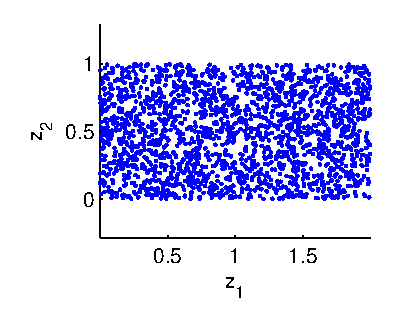
\includegraphics[height=2.5cm]{strip_data_L2}
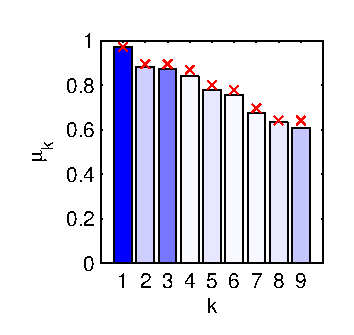
\includegraphics[height=3cm]{strip_spectrum_L2}
\caption{}
\end{subfigure}
%
%\hfill
%
\begin{subfigure}{0.25\textwidth}
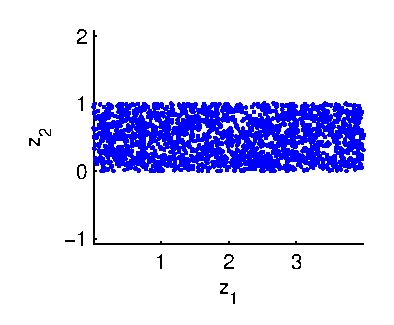
\includegraphics[height=2.5cm]{strip_data_L4}
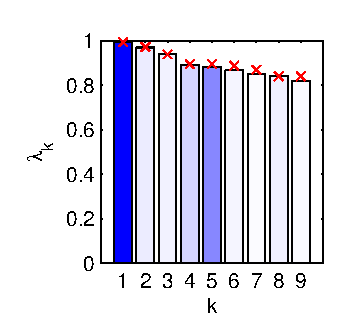
\includegraphics[height=3cm]{strip_spectrum_L4}
\caption{}
\end{subfigure}
%
%\hfill
%
\begin{subfigure}{0.3\textwidth}
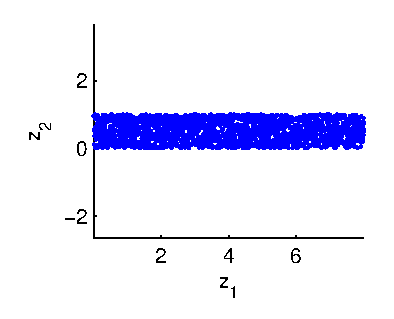
\includegraphics[height=2.5cm]{strip_data_L8}
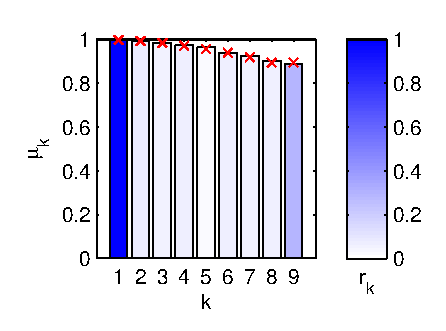
\includegraphics[height=3cm]{strip_spectrum_L8}
\caption{}
\end{subfigure}
%
\caption[Eigenvalues and eigenvectors of diffusion maps on a two-dimensional strip]{Data sets (top) and eigenvalue spectra from diffusion maps analysis (bottom) for strips with (a) $L_1 = 2$, $L_2 = 1$, (b) $L_1 = 4$, $L_2 = 1$, (c) $L_1 = 8$, $L_2 = 1$. The empirical eigenvalues are plotted in blue, and the analytical eigenvalues are plotted in red. From the eigenvalues which are identified as parametrizing unique eigendirections (indicated by the darker blue bars), the estimated length ratio from \eqref{eq:est_lengths} is (a) 2.2, (b) 4.1, (c) 8.7.}
\label{fig:strip_compare_analytic}
\end{figure}

Our first illustrative example consists of three different two-dimensional strip data sets.
%
Each data set contains $\ndata=2000$ data points uniformly sampled from the strip.
%
Figure~\ref{fig:strip_compare_analytic} shows the data sets and the diffusion maps eigenspectra.
%
The eigenvalues are colored by the leave-one-out cross-validation error as defined in \eqref{eq:cv_error}; a small value of $r_k$ indicates that the corresponding eigenvector is a repeated eigendirection, while a large value of $r_k$ indicates that the corresponding eigenvector describes a new direction in the data.
%

We observe that the eigenvalues are consistent with the known analytic eigenvalues of the Laplacian (see \eqref{eq:evals} and \eqref{eq:evals_relationship}), shown in red.
%
Furthermore, the two unique eigendirections can easily be identified, since their corresponding regression error $r_k$ is large.
%
As expected, the gap between the two meaningful eigenvalues increases as the strip becomes longer.
%
Using \eqref{eq:est_lengths}, we can accurately estimate the relative lengths of the two unique eigendirections in each data set.


\subsubsection{Swiss roll}

\begin{figure}[!t]
%
\begin{subfigure}{0.2\textwidth}
\centering
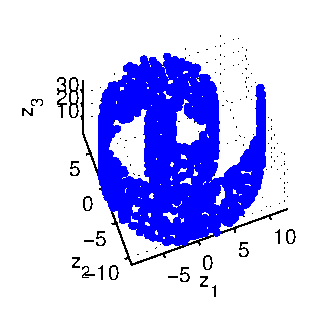
\includegraphics[width=\textwidth]{swissroll1}
\caption{}
\label{subfig:swissroll1}
\end{subfigure}
%
\begin{subfigure}{0.25\textwidth}
\centering
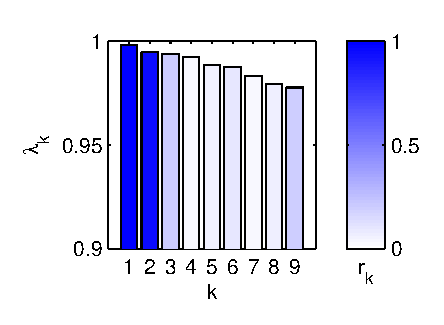
\includegraphics[width=\textwidth]{swissroll1_evals}
\caption{}
\label{subfig:swissroll1_evals}
\end{subfigure}
%
\begin{subfigure}{0.25\textwidth}
\centering
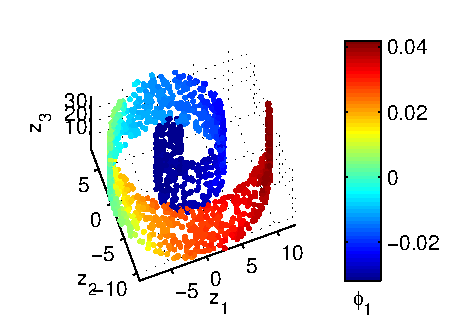
\includegraphics[width=\textwidth]{swissroll1_color1}
\caption{}
\label{subfig:swissroll1_color1}
\end{subfigure}
%
\begin{subfigure}{0.25\textwidth}
\centering
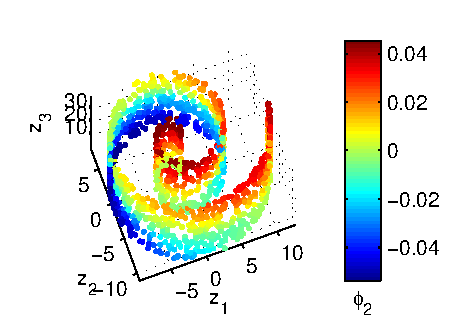
\includegraphics[width=\textwidth]{swissroll1_color2}
\caption{}
\label{subfig:swissroll1_color2}
\end{subfigure}

\begin{subfigure}{0.2\textwidth}
\centering
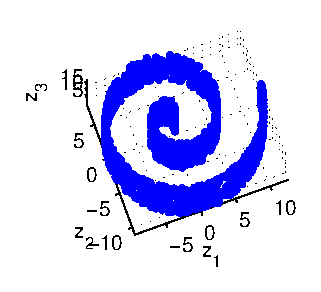
\includegraphics[width=\textwidth]{swissroll2}
\caption{}
\label{subfig:swissroll2}
\end{subfigure}%
%
\begin{subfigure}{0.25\textwidth}
\centering
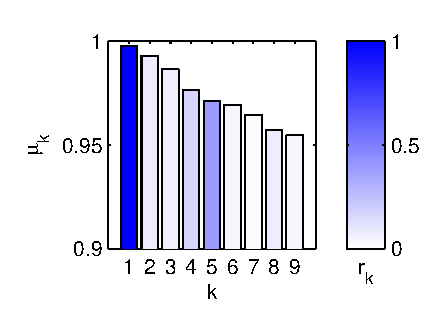
\includegraphics[width=\textwidth]{swissroll2_evals}
\caption{}
\label{subfig:swissroll2_evals}
\end{subfigure}
%
\begin{subfigure}{0.25\textwidth}
\centering
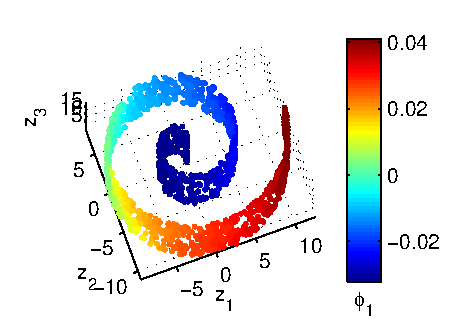
\includegraphics[width=\textwidth]{swissroll2_color1}
\caption{}
\label{subfig:swissroll2_color1}
\end{subfigure}
%
\begin{subfigure}{0.25\textwidth}
\centering
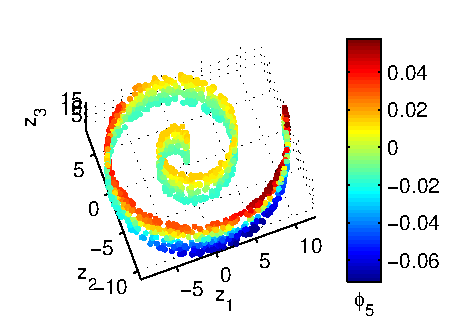
\includegraphics[width=\textwidth]{swissroll2_color2}
\caption{}
\label{subfig:swissroll2_color2}
\end{subfigure}
%
\caption[Eigenvalues and eigenvectors of diffusion maps on a swiss roll]{Swiss roll example. (a) Data set 1; $h= 40$. (b) Eigenvalue spectrum from the diffusion maps analysis of data set 1. (c) Data set 1, colored by the first diffusion maps eigenvector. (d) Data set 1, colored by the second diffusion maps eigenvector. (e) Data set 2; $h = 20$. (f) Eigenvalue spectrum from the diffusion maps analysis of data set 2. (g) Data set 2, colored by the first diffusion maps eigenvector. (h) Data set 2, colored by the fifth diffusion maps eigenvector. }
\label{fig:swiss_rolls}	
\end{figure}

Our second illustrative example consists of two different Swiss roll data sets.
%
The data are sampled according to
\begin{equation}
\begin{aligned}
z_1 =& \theta \cos \theta \\
z_2 =& \theta \sin \theta \\
z_3 =& h t
\end{aligned}
\end{equation}
%
where $\theta$ is sampled such that $z_1, z_2$ are uniformly sampled along the arclength of the spiral, and $t \sim Unif(0,1)$.
%
Note that, in this example, $z_1, z_2, z_3$ are the original data coordinates; however, the data lie on a two-dimensional manifold parametrized by the $\theta$ and $t$.
%
The height of the first Swiss roll is $h = 40$, while the height of the second is $h = 20$.
%
Each data set consists of $\ndata=1500$ points, shown in Figures~\ref{subfig:swissroll1}~and~\ref{subfig:swissroll2}.
%
%We expect to recover the eigenvector which parametrizes the height farther down in the spectrum for the second data set relative to the first, as this second data set is shorter.

Figures~\ref{subfig:swissroll1_evals}~and~\ref{subfig:swissroll2_evals} shows the eigenvalue spectra from the analysis of the two data sets.
%
Similar to Figure~\ref{fig:strip_compare_analytic}, the bars are colored by the leave-one-out cross-validation error, where a small value of $r_k$ indicates that the corresponding eigenvector is a repeated eigendirection.
%
From these plots, one can conclude that the first two eigenvectors $\phi_1$ and $\phi_2$ parametrize the first data set, while $\phi_1$ and $\phi_5$ parametrize the second.
%
Figures~\ref{subfig:swissroll1_color1},\ref{subfig:swissroll1_color2},\ref{subfig:swissroll2_color1},~and~\ref{subfig:swissroll2_color2} shows the two data sets, colored by the two eigenvectors identified as parametrizing the unique eigendirections.
%
As expected, these eigenvectors are one-to-one with the arc length along the spiral, and the height of the Swiss roll.

\subsubsection{Torus}

\begin{figure}[t]
\centering
\begin{subfigure}{1.5in}
\centering
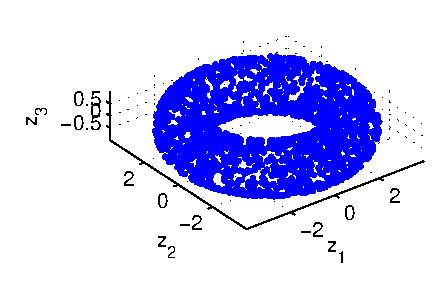
\includegraphics[height=0.75in]{torus1}
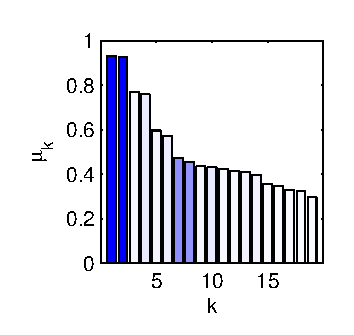
\includegraphics[height=1in]{torus1_evals}
\caption{}
\end{subfigure}
%
%\hfill
%
\begin{subfigure}{1.5in}
\centering
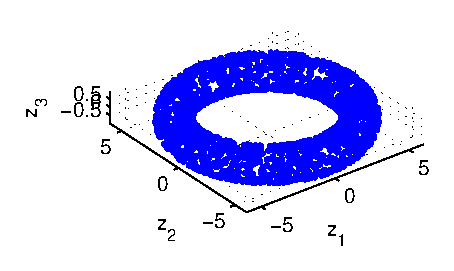
\includegraphics[height=0.75in]{torus2}
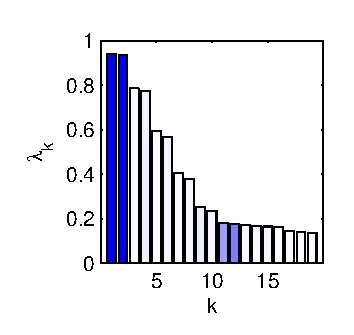
\includegraphics[height=1in]{torus2_evals}
\caption{}
\end{subfigure}
%
%\hfill
%
\begin{subfigure}{1.5in}
\centering
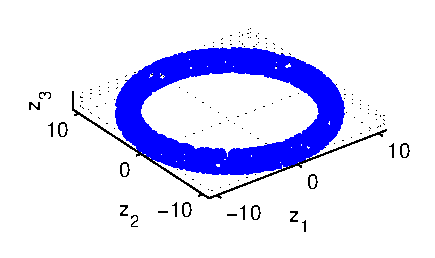
\includegraphics[height=0.75in]{torus3}
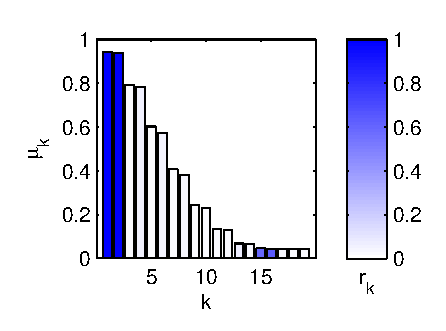
\includegraphics[height=1in]{torus3_evals}
\caption{}
\end{subfigure}
%
\hfill
%
\caption[Eigenvalues and eigenvectors of diffusion maps on a torus]{Torii data sets (top, see \eqref{eq:torus}) and corresponding diffusion maps eigenvalues (bottom) for (a) $r_1 = 3$, $r_2 = 1$. (b) $r_1 = 5$, $r_2 = 1$. (c) $r_1 = 10$, $r_2 = 1$. In all three data sets, the first two eigenvalues/eigenvectors correspond to $\sin \theta_1$ and $\cos \theta_1$. The second pair of unique eigendirections (corresponding to $\sin \theta_2$ and $\cos \theta_2$) are captured by components 7 and 8, 11 and 12, and 15 and 16, respectively.}
%
\label{fig:torus}
%
\end{figure}

For the third example, we consider a torus defined by
%
\begin{equation}
\begin{aligned}
z_1 =& (r_1 + r_2 \cos \theta_2 ) \cos \theta_1 \\
z_2 =& (r_1 + r_2 \cos \theta_2 ) \sin \theta_1 \\
z_3 =& r_2 \sin \theta_2
\end{aligned}
\label{eq:torus}
\end{equation}
%
where $r_1 > r_2$ are the outer and inner radii, respectively, and $\theta_1, \theta_2 \sim Unif(0, 2 \pi)$.
%
In this example, $z_1, z_2, z_3$ are the coordinates of the data; however, we expect to obtain from our analysis two eigenfunctions ($\sin \theta_1$ and $\cos \theta_1$) which parametrize the outer circle, and two eigenfunctions ($\sin \theta_2$ and $\cos \theta_2$) which parametrize the inner circle.
%
Intuitively, increasing $r_1$ can be viewed as analogous to increasing the ratio of $L_1$ to $L_2$ in the strip example and makes the eigendirections which parametrize the outer circle ($\cos \theta_1$ and $\sin \theta_1$) more dominant compared to the eigendirections with parametrize the inner circle.
%
Figure~\ref{fig:torus} shows the eigenspectra from the analysis of three different torii, colored by the leave-one-out cross-validation error.
%
We observe that as the torus becomes thinner ($r_1$ increases), the second pair of eigenvalues corresponding to unique eigendirections (corresponding to $\sin \theta_2$ and $\cos \theta_2$) moves farther down in the spectrum.

\section{Chemotaxis: A Case Study}

Our main motivation for identifying the unique eigendirections is to facilitate the analysis of complex data sets where the underlying structure is not readily apparent.
%
In data from complex dynamical systems, noisy microscopic behavior often gives rise to coherent macroscopic dynamics.
%
In general, this mapping from microscale to macroscale is not always obvious.
%
We will show how we can use our proposed methodology to extract a parametrization of data collected at the microscale which is consistent with the macroscopic behavior, without any {\em a priori} knowledge of the appropriate microscopic or macroscopic model.
%
Furthermore, determining the {\em true} dimensionality of such a parametrization by identifying the unique eigendirections reveals the requisite dimensionality of a reduced model which captures the relevant macroscopic behavior.
%
Knowing appropriate macroscopic variables and the true dimensionality can help inform modeling efforts and aid in the writing of accurate macroscale models.

Our model problem describes the process of cellular chemotaxis \cite{othmer2000diffusion}, where biological cells exhibit coherent macroscopic dynamics regulated by extracellular sensed signals in order to accomplish tasks such as finding food or navigating away from toxins.
%
Several microscopic models have been proposed to describe chemotaxis dynamics \cite{othmer1988models, codling2008random}.
%
We will analyze one such model described by a one-dimensional velocity jump process \cite{othmer2000diffusion}.
%
This specific example has an analytic macroscopic description in which the macroscopic dynamics of the group of cells depend on the value of a single system parameter.
%
This model serves as a ground truth and will allow us to verify our results which are obtained in an unsupervised manner.
%
Thus far, we only considered synthetic data sets for which the Euclidean distance between data points served as an informative metric.
%
Here, we will show that our approach, when utilizing the appropriate statistical observers and affinity metric between pairs of observations, uncovers a parametrization of the microscopic data which is consistent with the macroscopic model.
%
Furthermore, we will show that changes in dynamical behavior resulting from changes in the system parameters can be automatically detected.

\subsection{Problem description}

The microscopic model consists of a collection of $N$ cells (for our simulations, we take $N=1000$) whose states are defined by their positions and velocities on a line, and the dynamics of each cell are governed by a stochastic process.
%
Let $x_i(t)$ and $v_i(t)$ denote the position and velocity, respectively, of cell $i$ at time $t$.
%
The velocity of each cell is $\pm s$, where $s$ is a (fixed) speed.
%
We initialize the cells such that
\begin{equation}\label{eqn:system}
\begin{aligned}
x_i(0) & = 0 \\
\mathbb{P} \{ v_i(0) = +s \} & = p
\end{aligned}
\end{equation}
where $0 < p < 1$ is the probability of a cell initially moving to the right.
%
At random times, a cell will ``turn around'' and switch the direction of its velocity (this turning is controlled by extracellular signals).
%
The velocity of each cell randomly switches between $\pm s$ following an (independent) Poisson process with rate $\lambda_{switch}$.
%
For our specific simulations, we set $s^2/\lambda_{switch}=1$, which is consistent with the analysis presented in \cite{othmer1988models}.
%
We note that we have chosen a very specific one-parameter family of initial conditions which lead to simple dynamics and allow us to illustrate of our main points;
however, our analysis is not restricted to such specific cases and more complex initial conditions could be used.
%
Each data set consists of $10$ simulations, with initial conditions uniformly chosen such that $0.1 \le p  \le 0.9$.
%
We allow each simulation to evolve for $t_{max}$ time units with a fixed time step $dt$, and use data with $t > 0$ for analysis.

\begin{figure}[t!]
\def \figwidth {0.3\textwidth}
\centering
\begin{subfigure}{\figwidth}
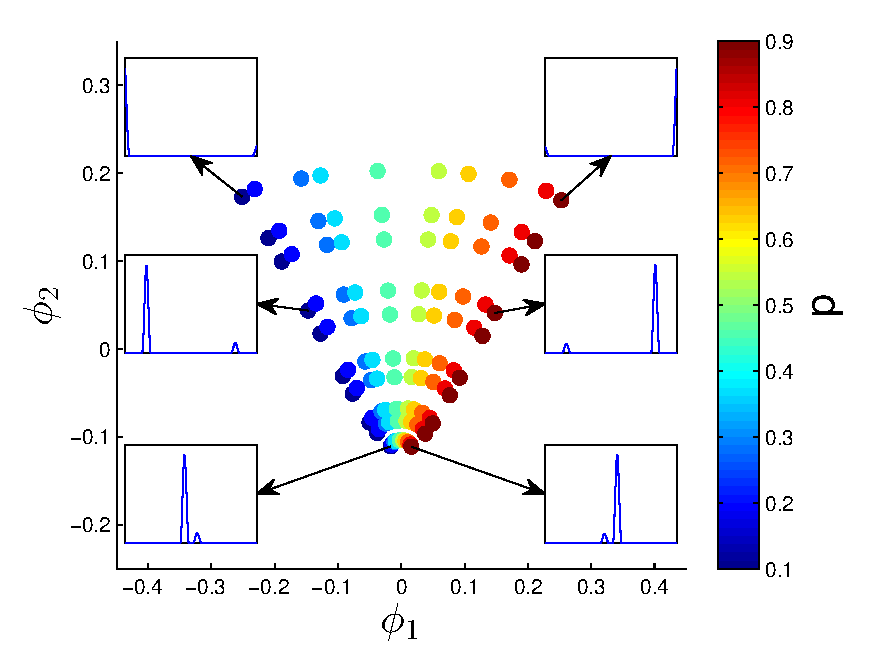
\includegraphics[width=\textwidth]{EMD_withhist_p_1}
\caption{}
\label{subfig:small_lambda_p}
\end{subfigure}
\begin{subfigure}{\figwidth}
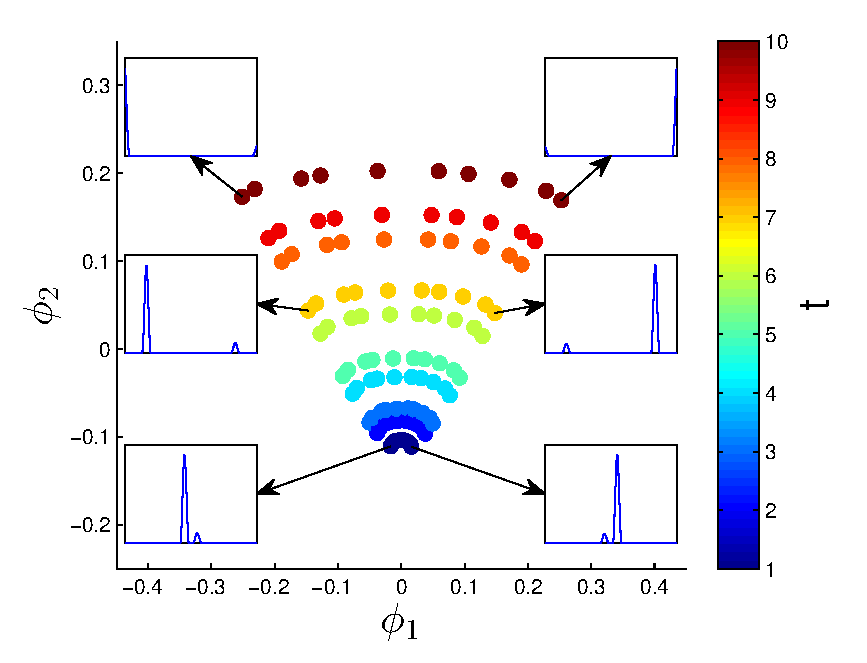
\includegraphics[width=\textwidth]{EMD_withhist_t_1}
\caption{}
\label{subfig:small_lambda_t}
\end{subfigure}
\begin{subfigure}{\figwidth}
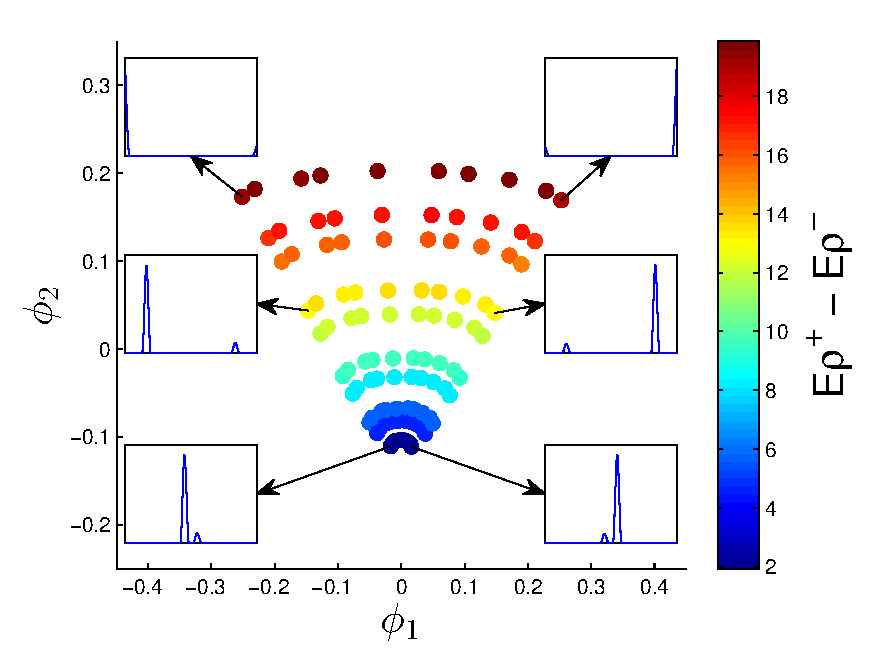
\includegraphics[width=\textwidth]{EMD_withhist_rho_1}
\caption{}
\label{subfig:small_lambda_rho}
\end{subfigure}

\begin{subfigure}{\figwidth}
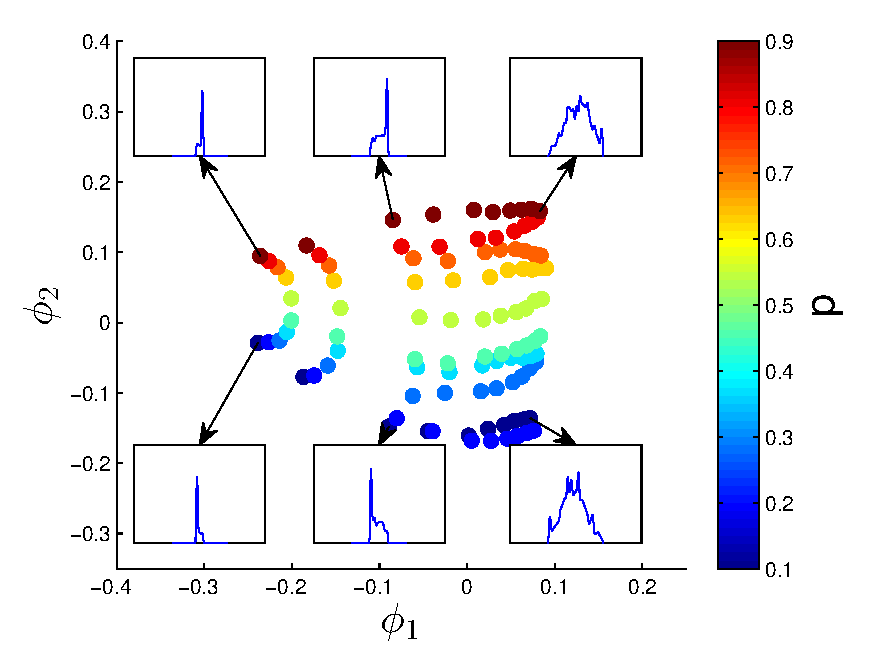
\includegraphics[width=\textwidth]{EMD_withhist_p_400}
\caption{}
\label{subfig:large_lambda_p}
\end{subfigure}
\begin{subfigure}{\figwidth}
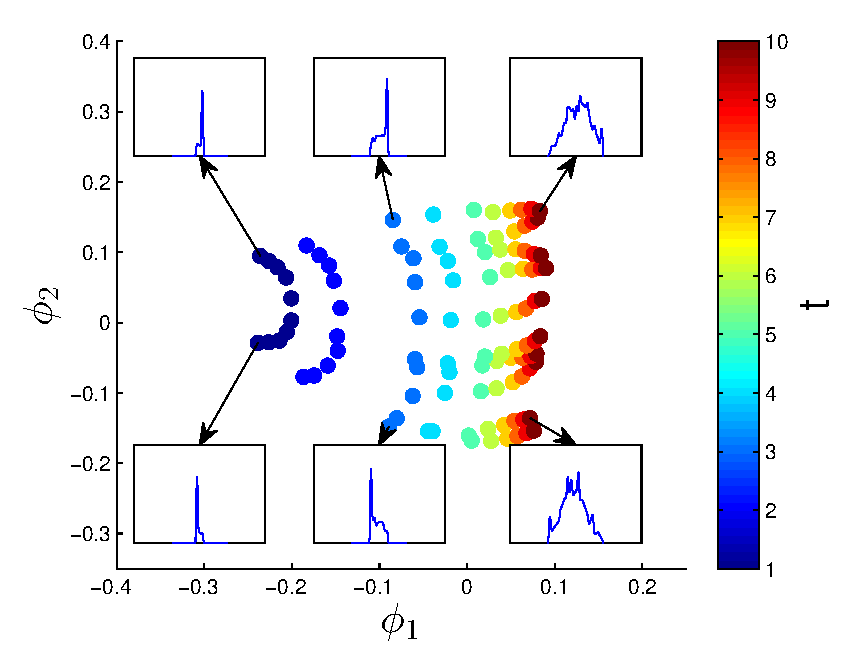
\includegraphics[width=\textwidth]{EMD_withhist_t_400}
\caption{}
\label{subfig:large_lambda_t}
\end{subfigure}
\begin{subfigure}{\figwidth}
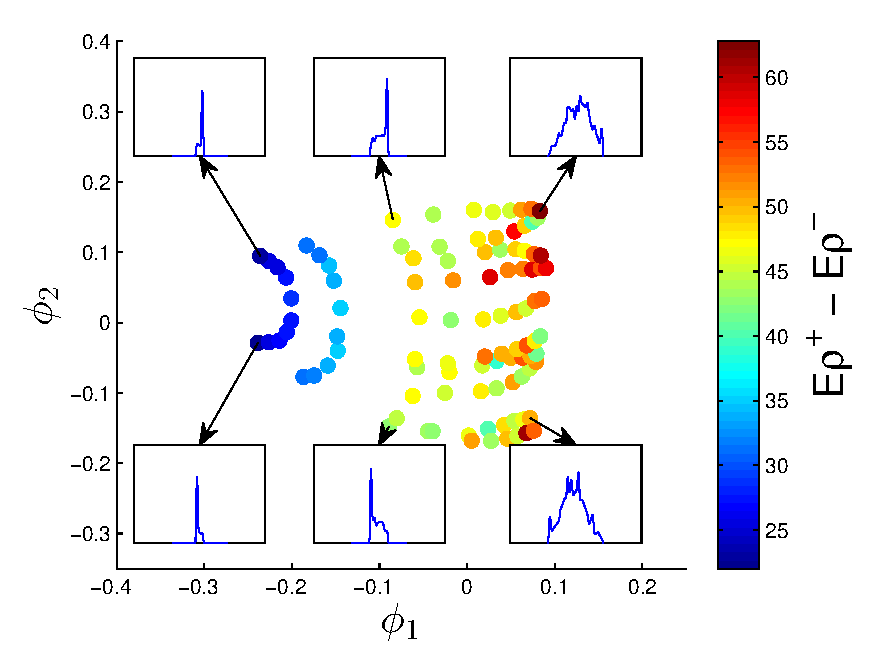
\includegraphics[width=\textwidth]{EMD_withhist_rho_400}
\caption{}
\label{subfig:large_lambda_rho}
\end{subfigure}
\caption[Diffusion maps embeddings of chemotaxis simulation data]{Embeddings using the first two diffusion maps eigenvectors computed from simulation data of the velocity jump process with (a--c) $\lambda_{switch}=1$, $s=1$, and (d--f) $\lambda_{switch}=400$, $s=20$.  We set $t_{max} = 10$ and $dt=1$. The distances used in the diffusion maps kernel are the earth mover's distances between the histograms of cell positions. The data are colored by (a, d) $p$, the initial probability of a cell moving to the right, (b, e) $t$, time, and (c, f) $E \rho^+ - E \rho^-$, the difference between the average position of the left- and right-moving cells. Representative histograms of the cell positions are shown for selected data points. }
\label{fig:dmaps_embed_emd}
\end{figure}

\subsection{Observers and metrics}

In general, manifold learning techniques have two essential components.
%
One is the appropriate {\em observers} of the system.
%
These observers should be informative as to the state of the system, as well as insensitive to noise in the system.
%
Two is a {\em distance metric} between the observations that captures a notion of locality: observations which we perceive to be similar should have a small distance.

For the chemotaxis example, we use histograms of the cell positions as observers.
%
Histograms are invariant to the indexing of the cells, while retaining information about the spatial locations of the cells.
%
Histograms are also robust to noise \cite{talmon2013empirical}.
%
Instead of the standard Euclidean distance, we use the earth mover's distance (EMD) \cite{rubner2000earth} as the metric between pairs of histograms.
%
Conceptually, the EMD measures how much ``work'' it takes to transform one probability density into another.
%
It therefore not only considers where the densities are inconsistent, but also how far apart the inconsistencies are.
%
Although the brute-force computation of the EMD is computationally expensive, there has been a plethora of work in developing efficient algorithms for its approximation \cite{Pele-eccv2008, Pele-iccv2009}.
%
For the specific case of one-dimensional data, the EMD is equivalent to the $L_1$-norm between the cumulative distribution functions of the data \cite{rubner2000perceptual}, which can be approximated from histograms as
\begin{equation}
\| \data(i) - \data(j) \|_{EMD} \approx \sum_{l=1}^{n} \left| \sum_{k=1}^l \data_k(i) - \sum_{k=1}^l \data_k(j) \right|,
\end{equation}
where the histograms $\data(i), \data(j)$ are defined on $\highdim$ equally-spaced bins in $\mathbb{R}$ (for our simulations, we will take $\highdim=32$), and $\data_k$ denotes the $k^{th}$ bin.
%
We note that although histograms are not essential to the theory of EMD, they make the computation feasible.


\subsection{Results}

\subsubsection{Identifying the unique eigendirections}

\begin{figure}[t]
\centering
\def\figheight{1.3in}
%
\begin{subfigure}[t]{1.5in}
\centering
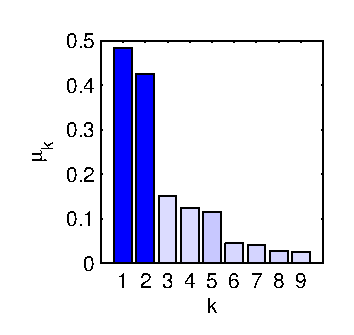
\includegraphics[height=\figheight]{chemotaxis1_evals}
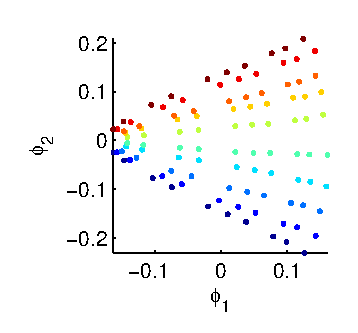
\includegraphics[height=\figheight]{chemotaxis1_embed_good}
\vspace{\figheight}
%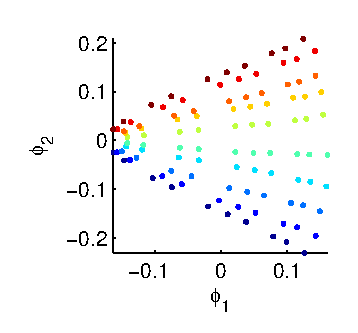
\includegraphics[height=1.5in]{chemotaxis1_embed_bad}
\caption{}
\end{subfigure}
%
\begin{subfigure}[t]{1.5in}
\centering
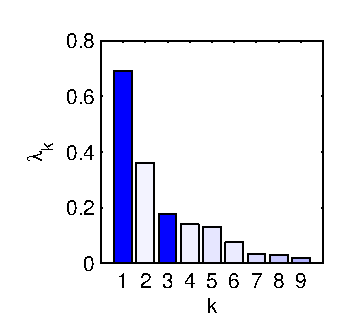
\includegraphics[height=\figheight]{chemotaxis2_evals}
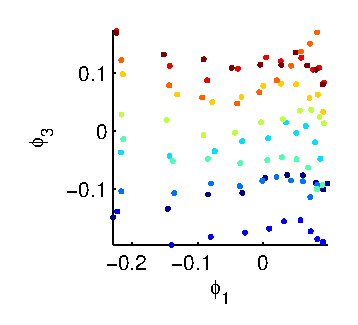
\includegraphics[height=\figheight]{chemotaxis2_embed_good}
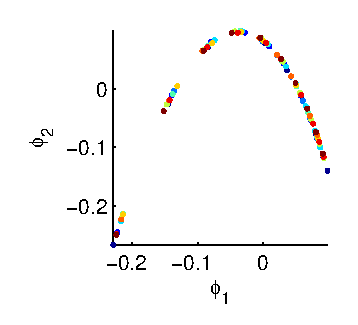
\includegraphics[height=\figheight]{chemotaxis2_embed_bad}
\caption{}
\end{subfigure}
%
\begin{subfigure}[t]{2in}
\centering
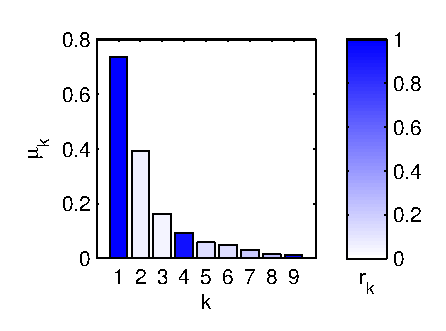
\includegraphics[height=\figheight]{chemotaxis3_evals}
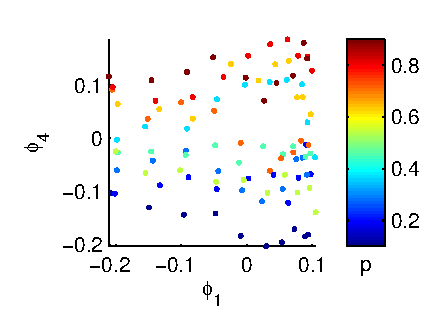
\includegraphics[height=\figheight]{chemotaxis3_embed_good}
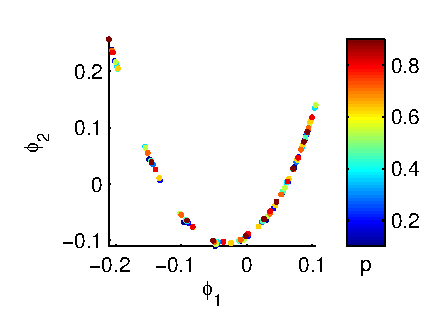
\includegraphics[height=\figheight]{chemotaxis3_embed_bad}
\caption{}
\end{subfigure}
%
\caption[Changes in diffusion maps eigenspectra for chemotaxis simulation data]{Analysis of three different chemotaxis simulation data sets. (a) $\lambda_{switch} = 100$, $s = 10$. (b) $\lambda_{switch} = 1600$, $s = 40$. (c) $\lambda_{switch} = 6400$, $s = 80$. We set $t_{max} = 10$ and $dt=1$, and the distances used in the diffusion maps kernel are the earth mover's distances between the histograms of cell positions. For each data set, the eigenvalue spectrum, colored by the cross-validation error, is shown in the top row. From the spectra, we can see that the first two components are informative for (a), components 1 and 3 are informative for (b), and components 1 and 4 are informative for (c). The corresponding reduced diffusion maps embeddings are shown in the middle row. For comparison, the standard diffusion maps embeddings using the first two components are also shown in the bottom row in (b) and (c).}
%
\label{fig:chemotaxis_simulations_harmonics}
\end{figure}

Figure~\ref{fig:dmaps_embed_emd} shows the results of analyzing two sets of chemotaxis simulations.
%
One set of simulations (Figures~\ref{subfig:small_lambda_p}--\ref{subfig:small_lambda_rho}) is for a small value of $\lambda_{switch}$, and the other set (Figures~\ref{subfig:large_lambda_p}--\ref{subfig:large_lambda_rho}) is for a large value of $\lambda_{switch}$.
%
For both sets of simulations, the macroscopic variables $p$, which controls the initial distribution of the cells, and $t$, the time, are well-correlated with the eigenvectors $\phi_1$ and $\phi_2$.
%
%In both cases, $\phi_1$ is significantly more important than $\phi_2$, as indicated by the separation between the first two eigenvalues (for the small $\lambda_{switch}$ case, $\lambda_{switch}_1 = 0.4828$, and $\lambda_{switch}_2 = 0.4287$, and for the large $\lambda_{switch}$ case, $\lambda_{switch}_1 = 0.6288$, and $\lambda_2 = 0.3236$).
%
The dominant coordinate $\phi_1$ is correlated with $p$ for the small $\lambda_{switch}$ case (Figure~\ref{subfig:small_lambda_p}), and correlated with $t$ for the large $\lambda_{switch}$ case (Figure~\ref{subfig:large_lambda_t}), indicating that the relative importance of $p$ and $t$ changes in the two simulations.
%
%TODO: should we mention fluxes here??

As illustrated in the synthetic data sets we discussed previously, the two leading eigenvectors are not guaranteed to correspond to unique eigendirections.
%
Figure~\ref{fig:chemotaxis_simulations_harmonics} shows the results of analyzing three different simulations which span a larger range of $\lambda_{switch}$ values compared to Figure~\ref{fig:dmaps_embed_emd}.
%
We see from the eigenspectra and the cross-validation errors $r_k$ that the second unique eigendirection moves down in the spectrum as $\lambda_{switch}$ increases.
%
The two-dimensional reduced diffusion maps embeddings obtained from eigenvectors which parametrize unique eigendirections capture the macroscopic variables $p$ and $t$ (we only show the correspondence of the two identified unique eigendirections with $p$ in the middle row of Figure~\ref{fig:chemotaxis_simulations_harmonics}; the correspondence between these eigendirections and $t$ is similarly consistent).
%
In contrast, the standard diffusion maps embeddings using the two leading eigenvectors $\phi_1$ and $\phi_2$ produce uninformative embeddings for large values of $\lambda_{switch}$, as $\phi_2$ is a repeated eigendirection which does not parametrize any new directions in the data.
%
Furthermore, although the eigenvalue spectra do not exhibit any large spectral gaps, the gap between the eigenvalues which correspond to new directions in the data (colored in blue) increases with $\lambda_{switch}$, indicating that the underlying manifold becomes more narrow/one-dimensional, and the corresponding eigenvectors provide us with an informative two-dimensional parametrization of the data. %which is consistent with the expected macroscopic dynamics.
%
It now becomes clear that looking at the eigenvectors {\em modulo} repeated eigendirections is essential for extracting an informative parametrization of the data, as well as characterizing the dimensionality of the data.

\subsubsection{Analytic macroscopic description}

This particular example has a known analytic macroscopic equation that governs the overall system behavior.
%
For a large collection of cells ($N \rightarrow \infty$), the system can be described by the probability density of the cells.
%
Let $\rho(x, t)$ denote the probability density of the cells, and let $\rho^-(x, t)$ and $\rho^+(x, t)$ denote the densities of the cells moving in the negative and positive axis directions, respectively.
%
It can be shown that, as $N \rightarrow \infty$, the densities satisfy the following set of partial differential equations (PDEs) \cite{othmer2000diffusion}:
\begin{equation} \label{eqn:coupled_pdes}
\begin{aligned}
\frac{\partial \rho^+}{\partial t} + s \frac{\partial \rho^+}{\partial x} & = -\lambda_{switch} \rho^+ +\lambda_{switch} \rho^- \\
\frac{\partial \rho^-}{\partial t} - s \frac{\partial \rho^-}{\partial x} & = \lambda_{switch} \rho^+ -\lambda_{switch} \rho^-
\end{aligned}
\end{equation}
%
Alternatively, \eqref{eqn:coupled_pdes} can be rewritten as one, second--order PDE:
\begin{equation} \label{eq:second_order_pde}
\frac{\partial^2 \rho}{\partial t^2} + 2 \lambda_{switch} \frac{\partial \rho}{\partial t} = s^2 \frac{\partial ^2 \rho}{\partial x^2}
\end{equation}
%
From \eqref{eq:second_order_pde}, we see that, for fixed values of $\lambda_{switch}$ and $s$, the macroscopic state of the system (the probability density of the cells) is indeed a function of the initial condition (parametrized by $p$) and the time $t$.
%
This implies that for fixed $\lambda_{switch}$ and $s$, the {\em microscopic} data in a high-dimensional ambient space (e.g., the positions of all $N$ cells) should lie on a two-dimensional manifold parametrized by $p$ (which controls the initial ratio of $\rho^+$ and $\rho^-$) and $t$ (which describes the evolution),
and uncovering the low-dimensional structure of the microscopic data reveals this manifold.
%
This is consistent with the results presented in Figures~\ref{fig:dmaps_embed_emd}~and~\ref{fig:chemotaxis_simulations_harmonics}, where the two-dimensional embeddings obtained from microscopic simulation data are one-to-one with $p$ and $t$.

We consider two asymptotic regimes of simulation.
%
When $\lambda_{switch} \rightarrow 0$, the right-hand side of \eqref{eqn:coupled_pdes} tends to 0, and \eqref{eqn:coupled_pdes} becomes two uncoupled wave equations,
\begin{equation}
\begin{aligned}
\frac{\partial \rho^+}{\partial t} + s \frac{\partial \rho^+}{\partial x} & = 0 \\
\frac{\partial \rho^-}{\partial t} - s \frac{\partial \rho^-}{\partial x} & = 0.
\end{aligned}
\end{equation}
%
When $\lambda_{switch} \rightarrow \infty$ with $s^2/\lambda_{switch}$ fixed, \eqref{eq:second_order_pde} approaches the heat equation,
\begin{equation}
2 \frac{\partial \rho}{\partial t} = D \frac{\partial ^2 \rho}{\partial x^2},
\end{equation}
%
where $D=s^2/\lambda_{switch}$.
%
The above analysis shows that the initial distribution of velocities of the cells (determined by $p$ in the microscopic simulations) plays a very different role depending on the value of $\lambda_{switch}$.
%
When $\lambda_{switch} \rightarrow 0$, the dynamics are described by two wave equations, and the initial distribution persists throughout the trajectory.
%
When $\lambda_{switch} \rightarrow \infty$, the dynamics are described by one heat equation, and the initial conditions are insignificant -- the velocity distribution quickly equilibrates and we see purely diffusive behavior.

The relative importance of $p$ and $t$ from the analytic description are consistent with the results in Figure~\ref{fig:dmaps_embed_emd}, where $p$ is correlated with the dominant coordinate when $\lambda_{switch}$ is small and correlated with the subdominant coordinate when $\lambda_{switch}$ is large.
%
Furthermore, in the small $\lambda_{switch}$ regime (wave equation), shown in Figures \ref{subfig:small_lambda_p}--\ref{subfig:small_lambda_rho}, the points corresponding to small times are more tightly clustered than the points corresponding to large times.
%
This is in agreement with the macroscopic model: at small times, the cells are more condensed around $x=0$, and it is more difficult to distinguish the cells moving to the left from the cells moving to the right.
%
On the other hand, at large times, once the cells evolve from the origin, this separation is clear.
%
For the large $\lambda_{switch}$ case (heat equation), shown in Figures \ref{subfig:large_lambda_p}--\ref{subfig:large_lambda_rho}, we observe that at small times, the initial distribution $p$ is well organized in the embedding in Figure \ref{subfig:large_lambda_p}, as the skew of the velocity distribution can be seen in the initial displacements.
%
On the other hand, for large times, we observe that the initial distribution $p$ is less organized in Figure \ref{subfig:large_lambda_p}, as the velocities have equilibrated and the initial distribution is less detectable in the cell density.
%
Overall, in both cases, we obtain, in an unsupervised data-driven manner, an accurate picture of the macroscopic variables that govern the system dynamics.

Furthermore, this analytic macroscopic description reveals that when $\lambda_{switch}$ is small, the system dynamics can be described by the two densities $\rho^+$ and $\rho^-$, and when $\lambda_{switch}$ is large, the dynamics are described by a single density $\rho = \rho^+ + \rho^-$.
%
Figures~\ref{subfig:small_lambda_rho}~and~\ref{subfig:large_lambda_rho} show the data, colored by the difference in the average position of the left- and right-moving cells.
%
Clearly, for small $\lambda_{switch}$, where both $\rho^+$ and $\rho^-$ are required to describe the dynamics, the data is organized by the differences in the two densities.
%
However, for large $\lambda_{switch}$, the two densities rapidly equilibrate, and negligible organization based on the differences between the two densities is visible.

%\subsubsection{Using an appropriate metric}

This analytic macroscopic description also allows us to emphasize the importance of using an appropriate distance metric.
%
We analyzed the two sets of simulation data from Figure~\ref{fig:dmaps_embed_emd} using the standard Euclidean distance between the histograms to compute the distances in \eqref{eq:dmaps_kernel}.
%
We empirically found that there is no appreciable correlation between the embedding coordinates and the macroscopic variables $p$ and $t$ (the correlations between the embedding coordinates and the governing macroscopic variables are all less than 60\%, with the correlations for the small $\lambda_{switch}$ case being less than 20\%)
%
%In contrast, the correlations between the embedding coordinates and the macroscopic variables when using EMD in the diffusion maps calculation are all greater than 80\%
, and so using a metric which accurately describes the distances between observations is essential for obtaining an informative parametrization of data.

\subsubsection{Detecting changes in dimensionality}

\begin{figure}[t]
%
\centering
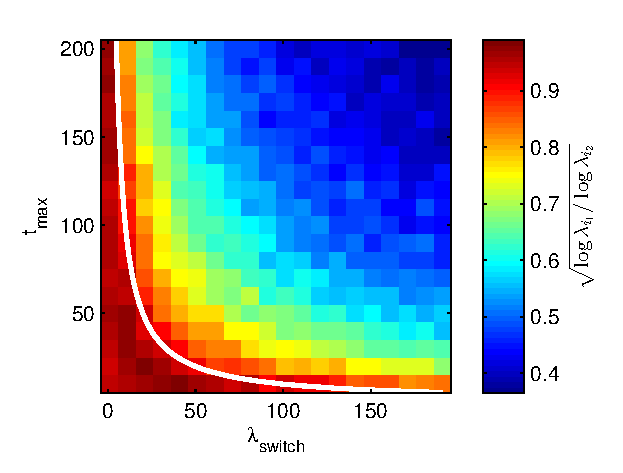
\includegraphics[width=0.5\textwidth]{tmax_lambda_transition}
%
\caption[Detecting changes in dimensionality of chemotaxis simulation data]{Detecting the change in dimensionality. The appropriate ratio the two eigenvalues (see \eqref{eq:chemotaxis_eval_ratio}) which correspond to unique eigendirections is plotted as a function of $t_{max}$ and $\lambda_{switch}$. Each data point is the average eigenvalue ratio over three replicate data sets, and in each simulation, $dt=t_{max}/10$. The distances used in the diffusion maps kernel are the earth mover's distances between the histograms of cell positions. The curve $1/\lambda_{switch} = t_{max}/N$ is shown in white. }
%
\label{fig:chemotaxis_compare_timescales_evals}
%
\end{figure}

Detecting changes in dimensionality is essential for the analysis and modeling of dynamical systems.
%
For this example, the true dimensionally of a data set can be estimated by looking at the two eigenvalues $\lambda_{i_1} \ge \lambda_{i_2}$ corresponding to unique eigendirections.
%
According to \eqref{eq:est_lengths}, we plot
\begin{equation}\label{eq:chemotaxis_eval_ratio}
 \sqrt{\frac{\log \lambda_{i_1}}{\log \lambda_{i_2}}} ;
\end{equation}
when this ratio becomes small, the data are effectively one-dimensional, as the second direction is very small compared with the first.

Figure~\ref{fig:chemotaxis_compare_timescales_evals} shows the eigenvalue ratio in \eqref{eq:chemotaxis_eval_ratio} as a function of $\lambda_{switch}$ and the time scale of observation $t_{max}$.
%
From this eigenvalue ratio, we detect changes in the estimated dimensionality as we vary the relevant parameters.
%
For small $\lambda_{switch}$ and/or short $t_{max}$, the data are effectively two-dimensional, as both $p$ and $t$ are important to the observed dynamics.
%
However, when $\lambda_{switch}$ and/or $t_{max}$ is large, the system rapidly equilibrates and the data are effectively one-dimensional, parametrized by $t$.
%
For this specific example, these changes are consistent with the analytically-predicted shift in the dynamical behavior at
\begin{equation}
\frac{t_{max}}{N} = \frac{1}{\lambda_{switch}}.
\end{equation}
%
This curve is also plotted in Figure~\ref{fig:chemotaxis_compare_timescales_evals} and is consistent with the transition predicted by the diffusion maps eigenvalues.

\section{Conclusions}

This paper addresses the issue of repeated eigendirections, one of the key shortcomings in applying diffusion maps analysis to real complex data.
%
We show that, using local linear regression, we can automatically detect which eigenvectors correspond to unique eigendirections in the data.
%
From this detection, we can then obtain a reduced diffusion maps embedding which is both parsimonious and induces a metric which is equivalent to the standard diffusion distance.
%
We then showed that these algorithms can allow us to analyze data from a complex dynamical system, enabling the extraction of good reduced coordinates and also the detection of changes in the dimensionality of the macroscopic dynamics.
%
In the future, we are confident that our proposed methodology will aid in the analysis of more complex data sets for which the dimensionality of the underlying manifold is unknown.